\documentclass[11pt]{article}

\usepackage[left=2cm,right=2cm,top=2cm,bottom=2cm]{geometry} 

\usepackage[utf8]{inputenc}   % otra alternativa para los caracteres acentuados y la "ñ"
\usepackage[           spanish % para poder usar el español
                      ,es-tabla % para los captions de las tablas
                       ]{babel}   
\decimalpoint %para usar el punto decimal en vez de coma para los números con decimales

%\usepackage{beton}
%\usepackage[T1]{fontenc}

\usepackage{parskip}
\usepackage{xcolor}

\usepackage{caption}

\usepackage{fancyvrb}

\usepackage{enumerate} % paquete para poder personalizar fácilmente la apariencia de las listas enumerativas

\usepackage{graphicx} % figuras
%\usepackage{subfigure} % subfiguras
\usepackage{subcaption}

\usepackage{amsfonts}
\usepackage{amsmath}

\usepackage{ marvosym }

\usepackage[formats]{listings}
\lstdefineformat{R}{~=\( \sim \)}
\lstset{basicstyle=\ttfamily,format=R}

\definecolor{gris}{RGB}{220,220,220}
	
\usepackage{float} % para controlar la situación de los entornos flotantes

\restylefloat{figure}
\restylefloat{table} 
\setlength{\parindent}{0mm}


\usepackage[bookmarks=true,
            bookmarksnumbered=false, % true means bookmarks in 
                                     % left window are numbered
            bookmarksopen=false,     % true means only level 1
                                     % are displayed.
            colorlinks=true,
            allcolors=blue,
            urlcolor=blue]{hyperref}
\definecolor{webblue}{rgb}{0, 0, 0.5}  % less intense blue


\title{\Huge Ataques Man-in-the-Middle \vspace{10mm}}

\author{\Large Grupo 1: \vspace{10mm} \\
	\Large David Cabezas Berrido \vspace{5mm} \\ 
  \Large dxabezas@correo.ugr.es \vspace{10mm} \\
  \Large Patricia Córdoba Hidalgo \vspace{5mm} \\ 
	\Large patriciacorhid@correo.ugr.es \vspace{10mm}}

\begin{document}
\maketitle
\vfill
\begin{flushleft}
{\Large Horas dedicadas al desarrollo de este trabajo: 20 aproximadamente}
\end{flushleft}
\vspace{40mm}
~
\newpage
\tableofcontents
\newpage

\section{Introducción}

Los ataques man-in-the-middel (MITM) son una clase de ciberataques en los que un individuo (el atacante) logra infiltrarse en una
comunicación entre dos partes legítimas, de forma que ambas partes ignoran su presencia. Esto permite al atacante acceder a información
de manera ilegítima, e incluso suplantar la identidad de alguno (o ambos) de los interlocutores y manipular el contenido de los mensajes. Es uno de los tipos de ciberataques más comunes, por lo que conviene estar informado sobre las distintas formas
en las que se manifiesta y saber cómo protegerse de él.

En esta memoria expondremos las características de este ataque, lo situaremos en su contexto histórico dentro del mundo de los ciberataques y la
 ciberseguridad, y facilitaremos algunos de los ejemplos reales de este ataque más notables a lo largo de la historia.
 
 También describiremos un método para comunicarse de forma segura evitando este tipo de ataque, el cifrado y firma de mensajes.
 
Además, realizaremos una simulación de este ataque en una red local que crearemos.

Finalmente, proporcionaremos una serie de consejos y buenas prácticas para evitar ser víctimas de este tipo de ataques.

\section{Preliminares}

El primer ataque MITM de la historia data del año 1903, y ocurrió durante una demostración del telégrafo inalámbrico de Marconi.
El Profesor Fleming, un asesor de Marconi, presentaba en el Royal Institute la recepción de un mensaje transmitido por Marconi desde la estación de
 Poldhu (a más de 400 kilómetros de distancia). Como la hora y el lugar de la demostración eran más que conocidos, el mago y fanático de la
tecnología Nevil Maskelyne logró interceptar uno de los mensajes y sustituirlo por un mensaje satírico. [\ref{bib-item-1}, \ref{bib-item-2}]

\begin{figure}[H]
	\centering
	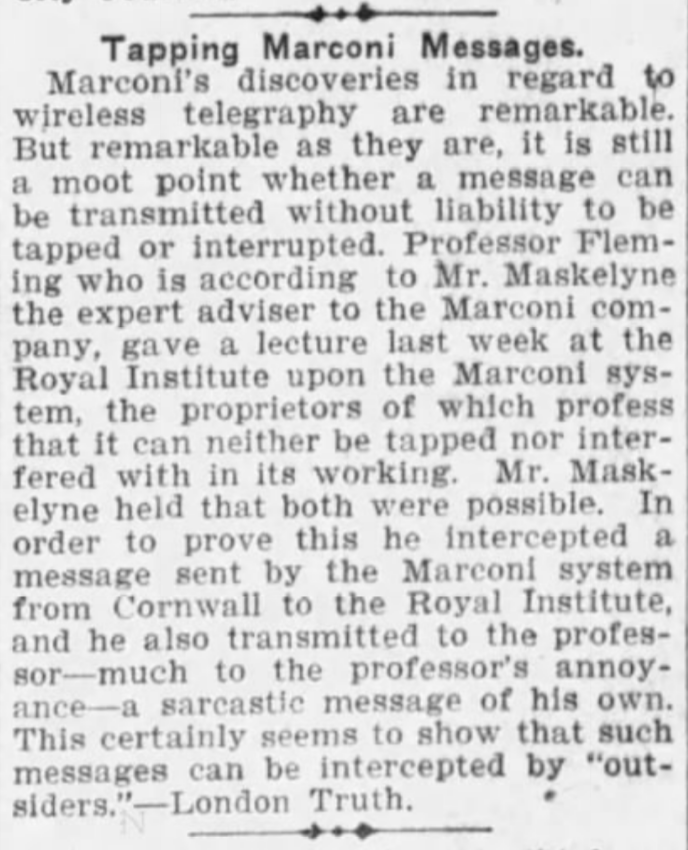
\includegraphics[width=75mm]{images/memoir/marconi-paper}
	\caption{Recorte de periódico: Austin-American Statesman, 17 de julio de 1903.}
\end{figure}

Con la extensión del uso de los ordenadores, este tipo de ataques cobró mucha popularidad a partir de la década de los 70. Una de las
primeras menciones a este tipo de ataques se encuentra en ``Software: A Qualitative Assessment, or The Man in the Middle Speaks Back'' (1973), por
Gerald H. Larsen. Leslie Lamport, desarrollador inicial de \LaTeX, escribió sobre cómo protegerse de este tipo de ataques en su artículo
``Password Authentication with Insecure Communication'' (1981). [\ref{bib-item-3}]

Para suscitar interés, exponemos a continuación algunos ejemplos notables de este tipo de ataque:
\begin{itemize}
	\item En 2013, Edward Snowden reveló que la NSA (US National Security Agency) se estaba haciendo pasar por Google para llevar un
	registro de las búsquedas de cada persona. Este ataque violaba gravemente el derecho a la intimidad de los ciudadanos, y se realizó con
	la excusa de combatir el terrorismo tras los sucesos del 11 de septiembre de 2001. Su poder para falsificar certificados SSL facilitó
	enormemente el ataque. [\ref{bib-item-4}]
	
	\item En 2015, un grupo de cibercriminales sustituyeron los datos bancarios en un e-mail que interceptaron a Paul Lupton, y que iba dirigido
	a la notaría para cobrar la venta de su piso. La cantidad de 333000 libras fue enviada a la cuenta fraudulenta en lugar de a la familia Lupton. [\ref{bib-item-5}]
	
	\item También en 2015, el ISP (Internet Service Provider) Comcast fue descubierto insertando anuncios y notificaciones en el contenido
	que sus clientes transmitían a través de su red. [\ref{bib-item-6}]
	
	\item Desde al menos finales de 2014, el Adware (software para incluir publicidad) de la empresa Superfish venía instalado en algunos ordenadores
	Lenovo. La instalación incluía la clave pública de Superfish en el equipo, y la usaba para volver a encriptar el tráfico después de desencriptarlo
	e introducir anuncios. Además, la clave pública era la misma para todos los equipos, y en cuanto se extrajo la clave privada, cualquiera podía
	emitir un certificado (para un sitio web o VPN) que todos estos ordenadores reconocerían como fiable. Esta polémica llevó al cierre de la empresa
	en mayo de 2015. [\ref{bib-item-7}]
	
	\item En 2017, una brecha de seguridad en las aplicaciones Android de varios bancos permitió el robo de credenciales a una gran cantidad de clientes
	a través de ataques MITM, sólo había que conectarse a la misma red que la víctima. [\ref{bib-item-8}]
	
	\item En 2010, un complemento de Firefox para recordar contraseñas utilizaba una cookie para que los usuarios no tuviesen que volver a introducir
	sus credenciales. Aunque el usuario y la contraseña eran cifrados, la cookie no, por lo que cualquiera que se hiciese con ella podría acceder
	a la cuenta del usuario de forma ilegítima. Este problema afectó sobre todo a Twitter y Facebook, y suscitó grandes esfuerzos por prevenir este tipo
	 de ataques en sitios web de esta índole. [\ref{bib-item-9}]
\end{itemize}

Como podemos observar, cada ataque aprovecha alguna brecha de seguridad o es perpetrado por una entidad con control sobre la red o sobre la autoridad
de certificación.

\section{Descripción del ataque Man-in-the-Middle}

La información de esta sección (salvo el ejemplo) la hemos extraído de [\ref{bib-item-10}] y [\ref{bib-item-11}], salvo
una parte de HTTPS Spoofing sofre dominios unicode, que aparece referenciada explícitamente.

Man-in-the-middle es un tipo de ciberataque en el que un atacante intercepta una comunicación entre dos entidades y se hace pasar por ambas a la vez.
Como resultado, ambos partícipes tienen la sensación de estar comunicándose directamente, cuando realmente la información puede ser
consultada y/o alterada por el atacante. 

Por ejemplo, imaginemos que el cliente Bob quiere conectarse a la aplicación del banco (el servidor) para hacer una trasferencia de 500\EUR \ al número de cuenta
xxx. Por desgracia, Alice (el atacante) logra interceptar la conexión por alguna de las formas que veremos más adelante, y recibe los credenciales de Bob para
acceder a la página del banco. Bob cree estar conectado a la aplicación del banco, cuando realmente está en una copia creada por Alice, mientras
que Alice se conecta a la aplicación (real) del banco usando los credenciales de Bob. De este modo, tanto Bob como el banco creen que se están
comunicando entre sí, pero ambos se están comunicando con Alice.

Cuando Bob rellena el (falso) formulario para realizar la transferencia de 500\EUR \ al número de cuenta xxx, Alice recibe este formulario y
rellena un formulario (real) en la aplicación del banco con la cuenta de Bob para hacer una transferencia de 5000\EUR \ al número de cuenta yyy,
el número de Alice. Como de costumbre, el banco envía un mensaje a Alice diciendo: ``Hola Bob, para confirmar su transferencia de 5000\EUR \ al número
 de cuenta yyy, sume los dígitos 1, 2 y 7 de su código secreto e introduzca el resultado''. Alice envía a Bob a través de la aplicación falsa
 un mensaje en el que dice:
 ``Hola Bob, para confirmar su transferencia de 500\EUR \ al número
 de cuenta xxx, sume los dígitos 1, 2 y 7 de su código secreto e introduzca el resultado''. El pobre Bob envía a Alice la respuesta de seguridad,
 sin saber que Alice la utilizará para robarle 5000\EUR. 
 
 Desde los puntos de vista de Bob y del banco, la comunicación que acaba de ocurrir corresponde al proceso normal de una transferencia. Sin embargo,
 Bob y el banco no han estado en contacto en ningún momento, y Alice ha sido la gran beneficiada. 
 Bob y el banco han sido víctimas de un ataque man-in-the-middle perpetrado por Alice.
 
 \begin{figure}[H]
 	\centering
 	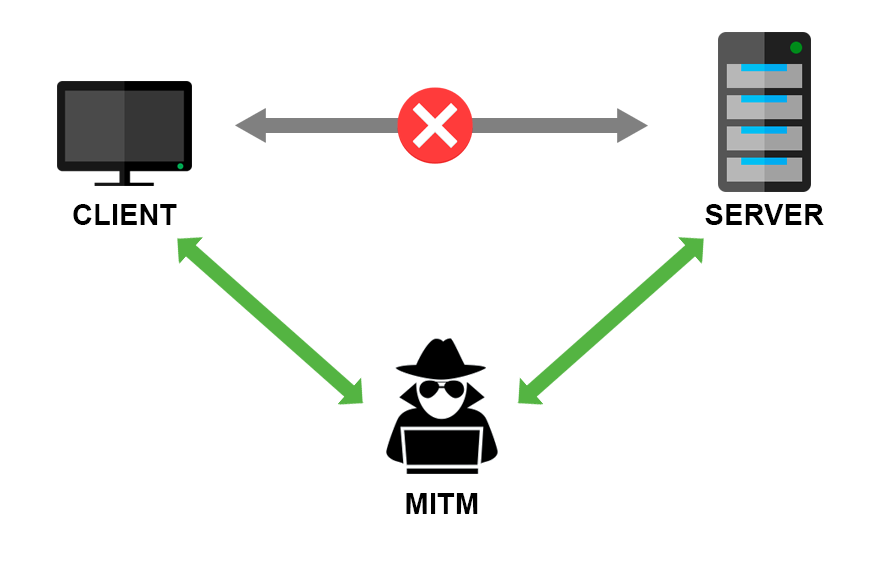
\includegraphics[width=120mm]{images/memoir/mitm}
 	\caption{Esquema de conexión típico de un ataque MITM. En este caso la comunicación es entre cliente y servidor, pero también podría
 		ser entre dos usuarios. \\ Fuente: \href{https://www.insicurezzadigitale.com/cose-un-attacco-man-in-the-middle}{https://www.insicurezzadigitale.com/cose-un-attacco-man-in-the-middle}.}
 \end{figure}
 
 Del mismo modo, este tipo de ataques pueden utilizarse para espiar conversaciones durante un largo tiempo, sin que ninguna de las partes legítimas
 se percate de ello.
 
 El inconveniente de los ataques man-in-the-middle es que requieren un papel muy activo del atacante, que debe reenviar los mensajes constantemente
 para las víctimas no sospechen que están siendo atacadas. Este proceso puede ser más o menos automatizable dependiendo de la medida en la que el
 atacante desee modificar la comunicación: puede simplemente escuchar y reenviar, o puede modificar los mensajes como en el ejemplo que acabamos
 de ilustrar.
 
 \subsection{Formas de hacer un ataque MITM}
 
 A continuación expondremos diferentes maneras de interceptar una comunicación y suplantar a ambos participantes. 
 
 \subsubsection*{ARP Cache Poisoning}
 
 El protocolo ARP es el encargado de relacionar cada dirección IP con la dirección física correspondiente. Para evitar tener que preguntar constantemente por la dirección física asociada una IP, este protocolo guarda en caché las direcciones físicas de las últimas direcciones IP consultadas.
 
 Un atacante puede beneficiarse de las características de este protocolo enviando a los integrantes de la comunicación mensajes en los que indique que la dirección IP del otro integrante corresponde con la dirección física del atacante. Así el atacante se infiltra en la conversación haciéndose pasar por ambas víctimas y recibiendo los mensajes que vayan destinados a cualquiera de las víctimas desde la otra. 
 
 Para que este ataque tenga éxito, es importante que el atacante siga mandando mensajes a sus víctimas y no corte la comunicación entre ambas, para que ninguna tenga la sospecha de que hay errores en el intercambio de información.
 
 \begin{figure}[H]
 	\centering
 	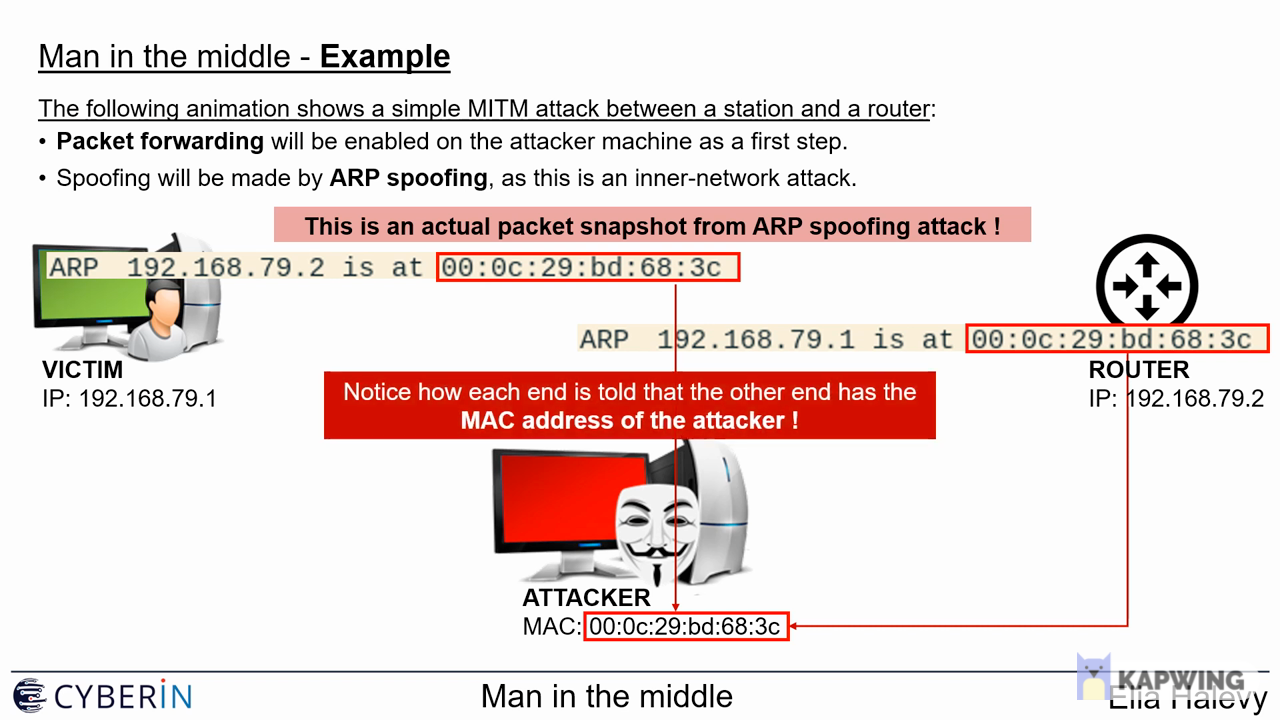
\includegraphics[width=120mm]{images/esquema-arp}
 	\caption{Esquema de ARP Cache Poisoning. Fotograma extraído de \href{https://www.youtube.com/watch?v=fbXu8EX0hsI}{este tutorial}.}
 \end{figure}

	Más adelante realizaremos una simulacción donde mostraremos cómo realizar un ataque MITM utilizando ARP Cache Poisoning.

\subsubsection*{DNS Cache Poisoning}

 El protocolo DNS tiene como función relacionar cada dominio con la dirección IP de la máquina que lo sirve. Cada máquina guarda en caché las direcciones IP de los últimos dominios visitados.
 
 El ataque MITM mediante DNS Cache Poisoning consiste en infiltrarse en la comunicación entre un usuario y un servidor DNS para proporcionarle al usuario una entrada DNS falsa que conduce a una página similar a la que éste quiere acceder. De este modo, el usuario piensa que está accediendo a una página cuando realmente navega en una creada por el atacante.
 
 \subsubsection*{HTTPS Spoofing}
 
 En este ataque, el atacante crea una página HTTPS con un dominio con apariencia similar al dominio de una de sus víctimas. Elabora la página de manera que su contenido sea idéntico al de la página original. De esta manera, el usuario que acceda a este dominio no sospechará de que la página no es segura, puesto que usa HTTPS y el dominio parece el mismo. Sin embargo, toda la información introducida en la página falsa podrá ser vista y usada posteriormente por el atacante.
 
 Por ejemplo, si visitamos el enlace \href{https://www.xn--80ak6aa92e.com}{https://www.xn--80ak6aa92e.com} veremos que el dominio que aparece en la
  barra de navegación se asemeja a \href{https://www.apple.com}{https://www.apple.com}, mientras que el contenido es totalmente distinto y ambas páginas
   utilizan HTTPS. [\ref{bib-item-12}]. Esto puede evitarse utilizando un navegador que maneje correctamente los dominios unicode o instalando alguna
  \href{https://github.com/yabirgb/punycodeAlert}{extensión} que detecte
 el uso de este tipo de dominios. Otra alternativa sería modificar la `a' de apple (en arabic) por una `a' del cirílico, ambos caracteres se ven
 igual, pero sus valores unicode son diferentes.
 
 Normalmente se utiliza el Phishing para hacer que la víctima haga click en uno de estos enlaces engañosos. Es decir, se le envía el link por email o mensaje de texto para intentar que entre. Una vez dentro, es muy complicado para la víctima percatarse de que la página web es ilegítima.
 
 \subsubsection*{Wi-Fi Eavesdropping}
 
 Los atacantes pueden interceptar el tráfico en redes públicas o inseguras, o incluso crear una red WiFi para ver todo el tráfico que circula por ella. Si un usuario escribe sus credenciales, contraseñas, cuentas bancarias o cualquier tipo de información sensible en esa red, el atacante puede robarlas y usarlas en su beneficio.
 
 \subsubsection*{Session Hijacking}
 
 Al iniciar la comunicación en una página web, se crea una cookie con información relativa a la sesión. Si un atacante es capaz de hacerse con dicha cookie, éste será capaz de navegar por dicha web haciéndose pasar por el usuario.

\section{Cifrado y firma para evitar ataques MITM}

Información extraída de [\ref{bib-item-13}].

Seguidamente, comentamos cómo el sistema de cifrado asimétrico puede ayudarnos a establecer un canal de comunicación libre de este tipo de ataque.
Todo lo que necesitamos es la seguridad de que el intercambio de claves públicas se haya realizado correctamente, ya sea en persona, por una
autoridad fiable que asigne las claves o por algún otro método seguro.

Imaginemos que Bob quiere enviar un mensaje a Eve. Primero Bob firmaría el mensaje cifrándolo con su clave privada, y a continuación lo cifraría
con la clave pública de Eve. Para descifrar el mensaje, Eve tendría que descifrarlo con su clave privada (algo que sólo Eve puede hacer) y posteriormente
lo descifraría con la clave pública de Bob. La única forma de que Eve obtenga un mensaje legible es que efectivamente sea Bob el que haya firmado el
 mensaje (con la clave privada de Bob) y lo haya cifrado para ella (con la clave pública de Eve).

Si el mensaje fuese interceptado por Alice, ésta no podría acceder a la información porque no dispone de la clave privada de Eve para descifrarlo,
y el mensaje simplemente se perdería si Eve no lo reenviase.
Además, es imposible que Alice pueda hacerse pasar por Bob, ya que si el mensaje no se firma cifrándolo con la clave privada de Bob (de la que Eve
tampoco dispone), Eve no obtendrá un mensaje legible al descifrarlo con la clave pública de Bob (comprobar la firma). Por tanto Eve sólo puede
reenviar el mensaje íntegro que recibió, sin siquiera poder leerlo.

Por supuesto, existen ocasiones en los que garantizar la seguridad del intercambio de claves es imposible. No conseguimos nada con este método si el
propio intercambio es interceptado por un atacante.

\section{Simulación de ataque}

A continuación, mostramos una simulación de un ataque Man-in-the-Middle, seguiremos
\href{https://www.youtube.com/watch?v=fbXu8EX0hsI}{este tutorial}. [\ref{bib-item-15}]

Creamos una nueva red local: \texttt{vboxnet1}. En ella tendremos los siguientes hosts:
\begin{itemize}
	\item Máquina anfitriona: El atacante. Tiene Ubuntu 20.04.2 LTS.
	\item Cliente: Una de las víctimas del ataque.
	\item Servidor: La otra víctima. Tiene el servicio de Apache2 básico, por el que sirve un \texttt{index.html} con el mensaje
	``Hellow World!''.
\end{itemize}

En la siguiente tabla podemos ver las direcciones (IP y MAC) de cada uno de los hosts.

\begin{table}[H]
	\centering
	\begin{tabular}{|c|c|c|}
		\hline
		\textbf{Host} & \textbf{IP}  & \textbf{MAC}      \\ \hline
		Atacante      & 192.168.57.1 & 0a:00:27:00:00:01 \\ \hline
		Cliente       & 192.168.57.3 & 08:00:27:01:3a:c8 \\ \hline
		Servidor      & 192.168.57.4 & 08:00:27:6c:b7:f2 \\ \hline
	\end{tabular}
	\caption{Direcciones de las máquinas en la red \texttt{vboxnet1}.}
	\label{tab:info-hosts}
\end{table}

\subsubsection*{Herramientas}

Instalamos las siguientes herramientas en la máquina atacante.

Debemos instalar \href{https://www.ettercap-project.org}{Ettercap}, un paquete con utilidades para este tipo de ataques.
Podemos hacerlo desde Ubuntu Software.

Para monitorizar el ataque utilizaremos Wireshark. También usaremos \texttt{urlsnarf} para husmear el tráfico HTTP entre las víctimas. Esta
herramienta muestra las las peticiones HTTP que se realizan. Para descargarla, utilizamos el comando \verb^sudo apt install dsniff^.

\subsubsection*{Ataque}

El primer paso es activar la redirección de paquetes en la máquina atacante. De otro modo, las víctimas no podrían comunicarse entre sí, ya
que los paquetes serían interceptados por el atacante, y se percatarían rápidamente del ataque. Podemos lograr esto ejecutando la orden
\verb|sysctl -w net.ipv4.ip_forward=1|, o escribiendo el valor 1 en el fichero \texttt{/proc/sys/net/ipv4/ip\_forward}. [\ref{bib-item-14}]

\begin{figure}[H]
	\centering
	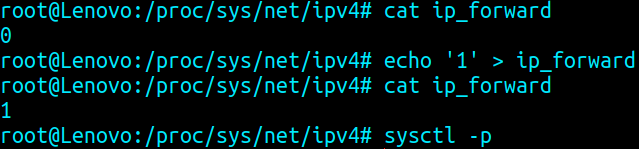
\includegraphics[width=110mm]{images/ip_forward}
	\caption{Activamos la redirección de paquetes escribiendo un 1 en el fichero \texttt{/proc/sys/net/ipv4/ip\_forward}.}
	\label{fig:ip_forward}
\end{figure}

Tras esto ejecutamos el comando \verb|sysctl -p| para hacer efectivos los cambios recién realizados.

Seguidamente, lanzamos Ettercap en el atacante, especificando el nombre de la interfaz de red que queremos atacar: \texttt{vboxnet1}.

\begin{figure}[H]
	\centering
	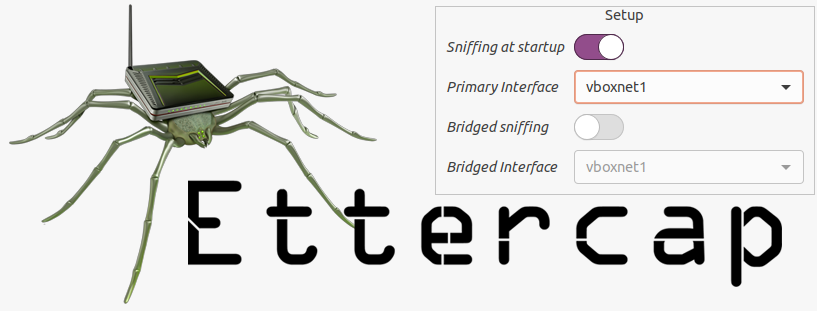
\includegraphics[width=140mm]{images/ettercap-start}
	\caption{Pantalla de inicio de Ettercap. Seleccionamos la red \texttt{vboxnet1}.}
	\label{fig:ettercap-start}
\end{figure}

Al entrar, recibimos los siguientes mensajes en la parte inferior de la ventana.

\begin{Verbatim}[tabsize=4]
Listening on:
vboxnet1 -> 0A:00:27:00:00:01
	192.168.57.1/255.255.255.0
	fe80::800:27ff:fe00:1/64

SSL dissection needs a valid 'redir_command_on' script in the etter.conf file
Ettercap might not work correctly. /proc/sys/net/ipv6/conf/all/use_tempaddr is not set to 0.
Ettercap might not work correctly. /proc/sys/net/ipv6/conf/vboxnet1/use_tempaddr is not set to 0.
Privileges dropped to EUID 65534 EGID 65534...

34 plugins
42 protocol dissectors
57 ports monitored
24609 mac vendor fingerprint
1766 tcp OS fingerprint
2182 known services
Lua: no scripts were specified, not starting up!
Starting Unified sniffing...
\end{Verbatim}

Podemos detener y reanudar el sniffing (husmeo) pulsando el botón de stop/play en la esquina
 superior izquierda. Este comienza activado.
 
Pulsamos en el botón \textit{Scan for hosts}, la lupa que se encuentra en la esquina superior izquierda, para buscar los host conectados a dicha interfaz. Al hacer esto nos aparece el siguiente mensaje en la parte inferior de la ventana:

\begin{Verbatim}[tabsize=4]
Randomizing 255 hosts for scanning...
Scanning the whole netmask for 255 hosts...
3 hosts added to the hosts list...
\end{Verbatim}

Podemos ver los hosts encontrados pulsando en el botón que aparece a la derecha de la lupa, \textit{Hosts List}.

\begin{figure}[H]
	\centering
	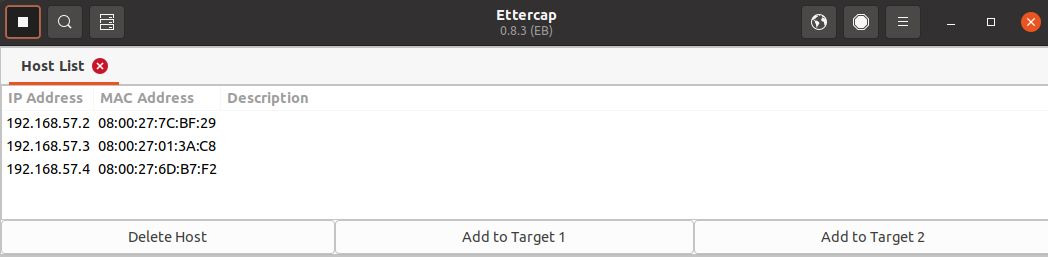
\includegraphics[width=140mm]{images/host-list}
	\caption{Lista de hosts conectados a la red \texttt{vboxnet1}.}
	\label{fig:host-list}
\end{figure}


Entre los hosts encontrados se encuentran nuestras dos víctimas. Seleccionamos el cliente, aquel con la dirección IP 192.168.57.3, y hacemos click en el botón \textit{Add to Target 1}. Análogamente seleccionamos el host con dirección IP 192.168.57.4 y hacemos click en el botón \textit{Add to Target 2}. Al hacer esto nos aparecen los siguientes mensajes en la ventana inferior.

\begin{Verbatim}
Host 192.168.57.3 added to TARGET1
Host 192.168.57.4 added to TARGET2
\end{Verbatim}

La otra dirección que aparece, 192.168.57.2, corresponde al router.

Una vez seleccionadas nuestras víctimas procedemos a envenenar la caché de ARP, es decir, desde el atacante se enviarán paquetes a ambas víctimas para que estas lo identifiquen como la víctima contraria. Para ello pulsamos el botón de \textit{MITM Menu}, aquel con el logo del globo terráqueo situado en la esquina superior derecha, y seleccionamos la opción \textit{ARP poisoning}. 

\begin{figure}[H]
	\centering
	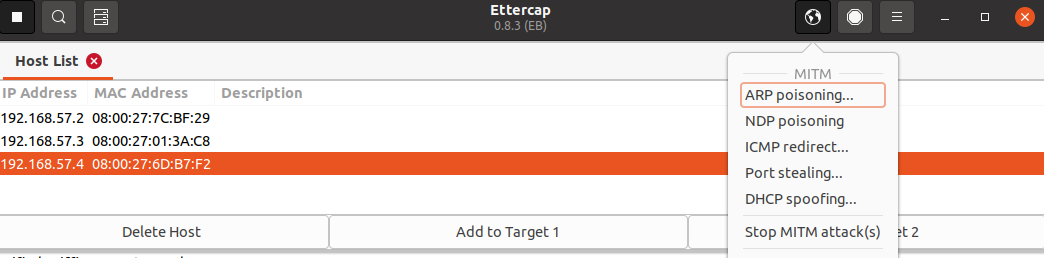
\includegraphics[width=140mm]{images/ettercap-mitm-arp-poisoning}
	\caption{Pulsamos en el botón \textit{MITM Menu}.}
	\label{fig:host-list}
\end{figure}

Nos aparece en una pantalla emergente con parámetros opcionales de esta funcionalidad. Marcamos el parámetro \textit{Sniff remote connections}.

\begin{figure}[H]
	\centering
	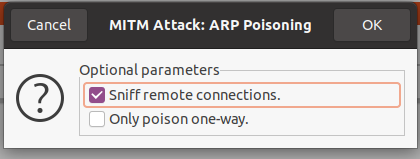
\includegraphics[width=90mm]{images/ettercap-arp-poisoning}
	\caption{Ventana emergente con las opciones de \textit{ARP poisoning}.}
	\label{fig:host-list}
\end{figure}

Obtenemos el siguiente mensage en la parte inferior de la ventana.

\begin{Verbatim}[tabsize=4]
ARP poisoning victims:

GROUP 1 : 192.168.57.3 08:00:27:01:3A:C8

GROUP 2 : 192.168.57.4 08:00:27:6D:B7:F2
\end{Verbatim}

Abrimos Wireshark y capturamos los paquetes de la interfaz \texttt{vboxnet1}. Podemos observar que se envían varios paquetes desde 0a:00:27:00:00:01, el atacante, a ambas víctimas. Por ejemplo, si nos fijamos en el primer paquete capturado podemos comprobar que es un paquete del atacante al cliente. Este paquete informa al cliente de que la dirección IP 192.168.57.4 se encuentra en la dirección MAC del atacante, cuando realmente esa dirección IP pertenece al servidor. Análogamente en el segundo paquete observamos como el atacante informa al servidor de que la dirección IP del cliente, 192.168.57.3, se encuentra en la dirección física del atacante.

Por tanto, el atacante ha conseguido que ambas víctimas le identifiquen como la contraria, por lo que todo el tráfico que circule entre ambas máquinas pasará por este y será capaz de husmearlo. Ha envenenado la caché de ARP.

\begin{figure}[H]
	\centering
	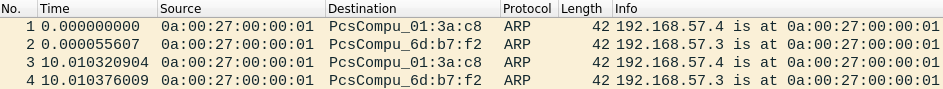
\includegraphics[width=140mm]{images/atack1/wireshark-arp}
	\caption{ARP poisoning. El atacante envía paquetes a sus víctimas con una identificación falsa.}
	\label{fig:wireshark-arp}
\end{figure}

Seguidamente, lanzamos \texttt{urlsnarf} en el atacante, indicando la interfaz de red con la opción \texttt{-i}. Esto nos permitirá
conocer las peticiones HTTP que se realicen entre el cliente y el servidor.

\subsubsection*{Análisis del tráfico}

El ataque ya está montado. Ahora hacemos CURL desde el cliente al servidor (\verb|curl http://192.168.57.4|).
Observamos la siguiente secuencia de intercambios en Wireshark.

\begin{figure}[H]
	\centering
	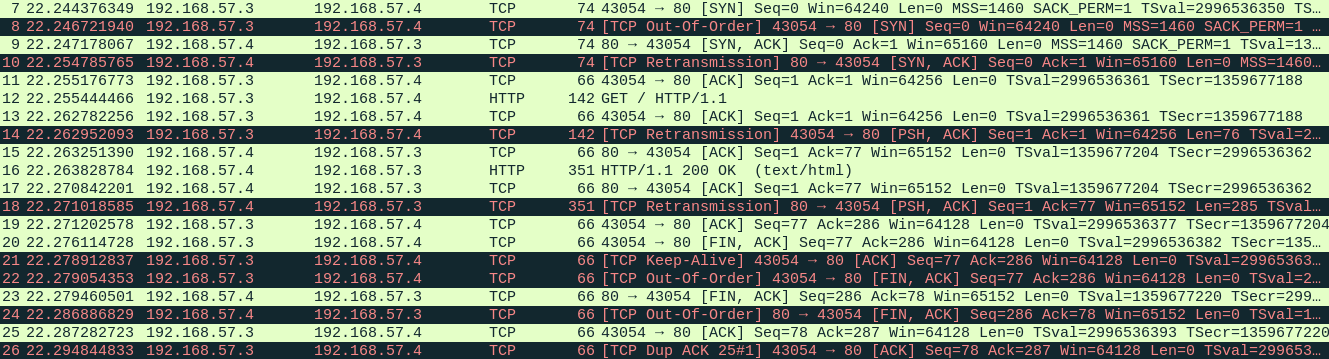
\includegraphics[width=170mm]{images/atack1/request}
	\caption{Comunicaciones capturadas mientras se realiza la petición.}
	\label{fig:request}
\end{figure}

Lo primero que nos llama la atención es la cantidad de paquetes \emph{Bad TCP}, que aparecen en negro y najanja. Esto
no es ningún fallo. Debido a que el atacante está actuando de intermediario, se realizan más intercambios de los esperados
entre las máquinas. A la hora de comprobar que la comunicación es correcta, Wireshark también piensa que el atacante es
una de las víctimas, de modo que la secuencia de paquetes que registra le confunde y piensa que se deben a errores en TCP. En 
seguida mostraremos ejemplos que reflejen esto.

Al analizar cualquiera de estos paquetes, tanto los relativos a la comunicación TCP (3-Way Handshake y cierre) como las peticiones y
respuestas HTTP, descubrimos que en ningún momento el cliente y el servidor consiguen comunicar directamente. A pesar de lo que aparece
en los campos IP origen e IP destino (tercera y cuarta columna), la dirección física de la máquina atacante aparece implicada
en cada transmisión. Observamos ésto analizando los paquetes 7 y 8, correspondientes a SYN. Podemos consultar las direcciones físicas en
la tabla \ref{tab:info-hosts}.

\begin{figure}[H]
	\centering
	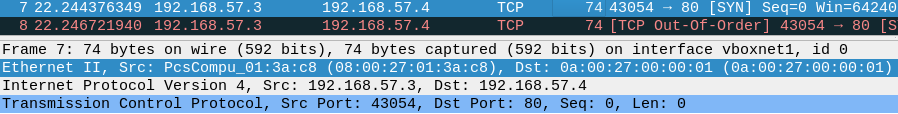
\includegraphics[width=160mm]{images/atack1/syn-client-atacker}
	\caption{Las direcciones IP y física de origen corresponden al cliente; y la dirección IP de destino es la del servidor. Sin embargo,
	la dirección física de destino realmente corresponde a la máquina atacante, que es la que realmente recibe el paquete. Esto se debe
	a un fallo en la caché de ARP del cliente, creado por el atacante. En nuestro caso, el paquete se reenvía a su verdadero destino,
	ya que activamos la redirección de paquetes, pero el atacante tiene la oportunidad de conocer el contenido.}
	\label{fig:syn-client-atacker}
\end{figure}

\begin{figure}[H]
	\centering
	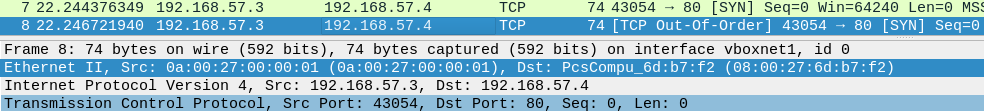
\includegraphics[width=160mm]{images/atack1/syn-atacker-server}
	\caption{El atacante reenvía el SYN al servidor y éste se piensa que procede del cliente debido a un error en la caché de ARP del servidor
		creado por el atacante. La dirección IP de origen es la del cliente y tanto la dirección IP como la dirección física de destino son las del servidor. La dirección física de origen es la del atacante. Puesto que Wiresharck interpreta que tanto el mensaje anterior como este son SYN que proceden de la misma IP y con la misma IP de destino piensa que se ha podido producir algún error durante el 3-Way Handshake. Por esto, señala este segundo paquete como \textit{Bad TCP} (Out-Of-Order).}
	\label{fig:syn-atacker-server}
\end{figure}

Analizamos ahora los paquetes correspondientes a la petición HTTP que se realiza de la máquina cliente al servidor. 

\begin{figure}[H]
	\centering
	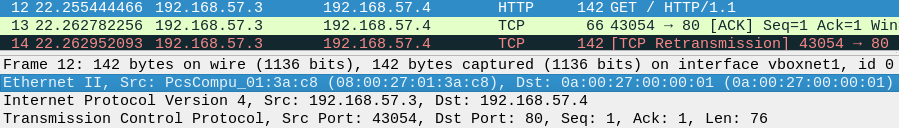
\includegraphics[width=160mm]{images/atack1/request-client-atacker}
	\caption{El cliente pretende mandar una petición HTTP al servidor. Podemos observar que la dirección IP y física de origen corresponden al cliente. La dirección IP de destino es la del servidor, pero la dirección física es la del atacante, luego realmente es al atacante al que se le manda la petición HTTP.}
	\label{fig:request-client-atacker}
\end{figure}

\begin{figure}[H]
	\centering
	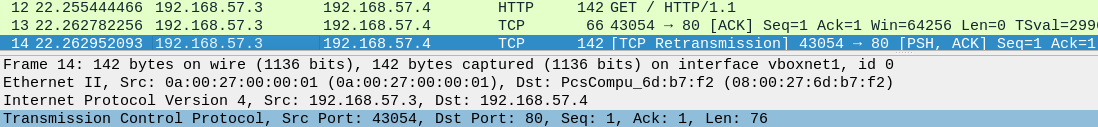
\includegraphics[width=160mm]{images/atack1/request-atacker-server}
	\caption{El atacante redirecciona la petición HTTP recibida al servidor. }
	\label{fig:request-atacker-server}
\end{figure}

\begin{figure}[H]
	\centering
	\begin{subfigure}{0.45\textwidth}
		\centering
		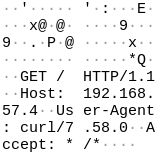
\includegraphics[width=30mm]{images/atack1/client-atacker}
		\captionsetup{width=0.5\linewidth}
		\caption{Contenido del paquete del cliente al atacante.}
	\end{subfigure}
	\hspace{-20mm}
	\begin{subfigure}{0.45\textwidth}
		\centering
		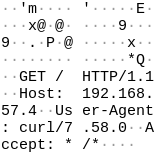
\includegraphics[width=30mm]{images/atack1/atacker-server}
		\captionsetup{width=0.5\linewidth}
		\caption{Contenido del paquete del atacante al servidor.}
	\end{subfigure}
	\caption{En el contenido del paquete podemos ver la petición HTTP mandada.}
\end{figure}

Del mismo modo, podemos analizar los paquetes de respuesta de la petición del servidor al cliente.

\begin{figure}[H]
	\centering
	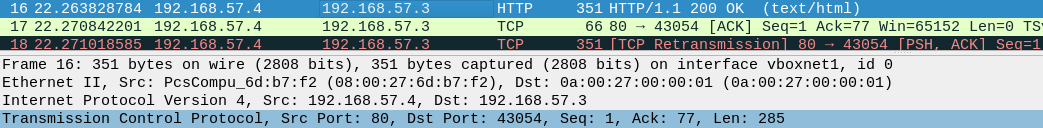
\includegraphics[width=160mm]{images/atack1/response-server-atacker}
	\caption{Como ocurre en el resto de paquetes, el servidor manda los paquetes cuya dirección IP de destino es el cliente a la dirección física del atacante. Así, el atacante puede husmear el contenido de los paquetes.}
	\label{fig:response-server-atacker}
\end{figure}

\begin{figure}[H]
	\centering
	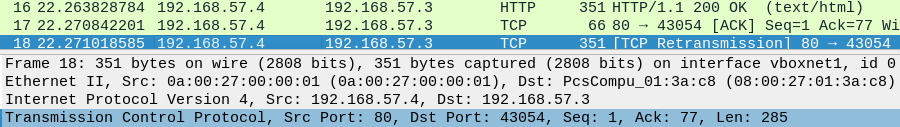
\includegraphics[width=160mm]{images/atack1/response-atacker-client}
	\caption{El atacante redirecciona el paquete recibido (la respuesta de la petición HTTP) al cliente.}
	\label{fig:response-atacker-client}
\end{figure}

\begin{figure}[H]
	\centering
	\begin{subfigure}{0.45\textwidth}
		\centering
		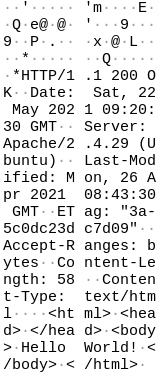
\includegraphics[width=30mm]{images/atack1/server-atacker}
		\captionsetup{width=0.5\linewidth}
		\caption{Contenido del paquete del servidor al atacante.}
	\end{subfigure}
	\hspace{-20mm}
	\begin{subfigure}{0.45\textwidth}
		\centering
		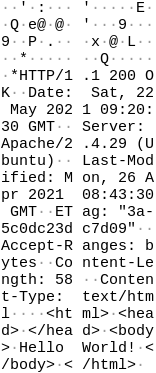
\includegraphics[width=30mm]{images/atack1/atacker-client}
		\captionsetup{width=0.5\linewidth}
		\caption{Contenido del paquete del atacante al cliente.}
	\end{subfigure}
	\caption{En el contenido del paquete podemos ver la respuesta de la petición HTTP mandada.}
\end{figure}

Además, \texttt{urlsnarf} registra cada petición HTTP que se haga entre las víctimas. Aparece una entrada por cada petición.

\begin{figure}[H]
	\centering
	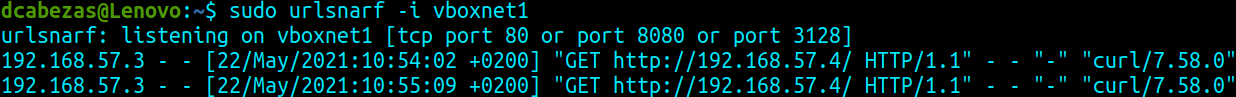
\includegraphics[width=160mm]{images/atack1/urlsnarf}
	\caption{Aparece una entrada por cada petición HTTP entre las víctimas.}
	\label{fig:urlsnarf}
\end{figure}

\section{Conclusiones}

Con este trabajo, esperamos haber concienciado al lector de la facilidad con la que se puede ser víctima de este tipo de ataques, así como
de la gravedad que pueden llegar a tener. La mayoría pueden encontrarse en [\ref{bib-item-16}], pero algunas las hemos deducido
del resto del contenido de este documento.

Notemos que es muy sencillo realizar un ataque man-in-the-middle cuando existe alguna brecha de seguridad. También cuando se tiene cierto poder
o control sobre la red o la autoridad de certificación.

Para finalizar, proporcionaremos algunas recomendaciones y buenas prácticas para evitar ser víctima de este tipo de ataques.
\begin{itemize}
	\item Evitar el uso de redes Wi-Fi públicas y sin contraseña.
	\item Evitar hacer logins en páginas (como una red social, tienda online o aplicación bancaria) desde redes públicas como las de cafeterías
	o bibliotecas.
	\item Evitar navegar en sitios web que no utilicen protocolo HTTPS, deberíamos tener un navegador que nos avise antes de entrar a una página que
	no lo utiliza.
	\item Usar varios factores de autenticación, lo que dificultará que nos perjudiquen con el robo de credenciales.
	\item Utilizar algún protocolo de cifrado y firma para intercambiar mensajes importantes.
	\item Cerrar la sesión en páginas antes de cerrarlas.
	\item Seguir el principio de \href{https://www.csoonline.com/article/3247848/what-is-zero-trust-a-model-for-more-effective-security.html}{confianza cero}: No aceptar conexiones hasta verificar su procedencia. [\ref{bib-item-17}]
\end{itemize}

Los siguientes comportamientos podrían indicar que estamos sufriendo un ataque MITM.
\begin{itemize}
	\item Experimentamos retrasos en la comunicación, o desconexiones inesperadas.
	\item Aparecen direcciones extrañas en nuestra barra de navegación.
	\item Tenemos conexiones a sitios desconocidos.
\end{itemize}

Si se diese el caso, podríamos confirmarlo y/o solucionarlo con las siguientes acciones.
\begin{itemize}
	\item Monitorizar la actividad de red con Wireshark o similares.
	\item Inspeccionar las conexiones actuales.
	\item Usar un network sniffer (una herramienta para espiar tráfico) de forma defensiva.
	\item Buscar software malicioso en nuestro equipo.
\end{itemize}

\section{Bibliografía}

Ataque MTIM en demostración de Marconi.
\begin{enumerate}
	\item \label{bib-item-1} \href{https://havocshield.com/2020/07/cybersecurity-history-the-very-first-man-in-the-middle-attack}{https://havocshield.com/2020/07/cybersecurity-history-the-very-first-man-in-the-middle-attack}.
	\item \label{bib-item-2} \href{https://www.bbc.com/mundo/noticias/2016/05/160523_primer_hacker_caballero_victoriano_marconi_fleming_maskelyne_finde_dv}{https://www.bbc.com/mundo/noticias/2016/05/\\160523\_primer\_hacker\_caballero\_victoriano\_marconi\_fleming\_maskelyne\_finde\_dv}.
\end{enumerate}

Primeras menciones a este tipo de ataques:
\begin{enumerate}
	\setcounter{enumi}{2}
	\item \label{bib-item-3} \href{https://www.apriorit.com/dev-blog/526-mitm-attacks-ssl-tls}{https://www.apriorit.com/dev-blog/526-mitm-attacks-ssl-tls}.
\end{enumerate}

Ejemplos notables.
\begin{enumerate}
	\setcounter{enumi}{3}
	\item\label{bib-item-4} Escándalo de la NSA: \href{https://www.cnet.com/news/nsa-disguised-itself-as-google-to-spy-say-reports}{https://www.cnet.com/news/nsa-disguised-itself-as-google-to-spy-say-reports}.
	\item\label{bib-item-5} Estafa a la familia Lupton: \href{https://www.conveyancingassociation.org.uk/fraudsters-hacked-emails-to-my-solicitor-and-stole-340000-from-my-property-sale-a-case-study-from-ca-affiliate-members-lawyer-checker}{https://www.conveyancingassociation.org.uk/fraudsters-hacked-emails-to-my-solicitor-and-stole-340000-from-my-property-sale-a-case-study-from-ca-affiliate-members-\\lawyer-checker}.
	\item\label{bib-item-6} Fraude de Comcast: \href{https://www.infoworld.com/article/2925839/code-injection-new-low-isps.html}{https://www.infoworld.com/article/2925839/code-injection-new-low-isps.html}.
	\item\label{bib-item-7} Incidente de Superfish con Lenovo: \href{https://www.techrepublic.com/article/superfish-adware-weakens-security-and-injects-ads-on-some-lenovo-laptops}{https://www.techrepublic.com/article/superfish-adware-weakens-security-and-injects-ads-on-some-lenovo-laptops}.
	\item\label{bib-item-8} Vulnerabilidad en aplicaciones bancarias: \href{https://www.zdnet.com/article/man-in-the-middle-flaw-left-smartphone-banking-apps-vulnerable}{https://www.zdnet.com/article/man-in-the-middle-flaw-left-smartphone-banking-apps-vulnerable}.
	\item\label{bib-item-9} Brecha de seguridad de Firesheep: \href{https://techcrunch.com/2010/10/24/firesheep-in-wolves-clothing-app-lets-you-hack-into-twitter-facebook-accounts-easily}{https://techcrunch.com/2010/10/24/firesheep-in-wolves-clothing-app-lets-you-hack-into-twitter-facebook-accounts-easily}.
\end{enumerate}

Ataque MITM: Explicación y tipos.
\begin{enumerate}
	\setcounter{enumi}{9}
	\item\label{bib-item-10} What is a MITM Attack, Detection and Prevention Tips: \href{https://www.varonis.com/blog/man-in-the-middle-attack}{https://www.varonis.com/blog/man-in-the-middle-attack}.
	\item\label{bib-item-11} A Review of Man-in-the-Middle Attacks: \href{https://arxiv.org/pdf/1504.02115.pdf}{https://arxiv.org/pdf/1504.02115.pdf}.
	\item\label{bib-item-12} Punycode alert: \href{https://github.com/yabirgb/punycodeAlert}{https://github.com/yabirgb/punycodeAlert}.
\end{enumerate}

Cifrado y firma para evitar ataques MITM.
\begin{enumerate}
	\setcounter{enumi}{12}
	\item\label{bib-item-13} Asignatura Seguridad y Protección de Sistemas Informáticos. Apuntes del profesor Francisco Miguel García Olmedo.
\end{enumerate}

Simulación.
\begin{enumerate}
	\setcounter{enumi}{13}
	\item\label{bib-item-14} Redirección de paquetes: \href{https://www.garron.me/es/gnu-linux/habilitar-ip-forward-linux-ubuntu.html}{https://www.garron.me/es/gnu-linux/habilitar-ip-forward-linux-\\ubuntu.html}.
	\item\label{bib-item-15} Tutorial YouTube: \href{https://www.youtube.com/watch?v=fbXu8EX0hsI}{https://www.youtube.com/watch?v=fbXu8EX0hsI}.
\end{enumerate}

Consejos para evitar ser víctimas del ataque.
\begin{enumerate}
	\setcounter{enumi}{15}
	\item\label{bib-item-16} What is a MITM Attack, Detection and Prevention Tips: \href{https://www.varonis.com/blog/man-in-the-middle-attack}{https://www.varonis.com/blog/man-in-the-middle-attack}.
	\item\label{bib-item-17} Zero Trust: \href{https://www.csoonline.com/article/3247848/what-is-zero-trust-a-model-for-more-effective-security.html}{https://www.csoonline.com/article/3247848/what-is-zero-trust-a-model-for-more-effective-security.html}.
\end{enumerate}

\end{document}
